\section{Introduction}
In the effort to accurately model physical phenomena using numerical methods,
one chief tool for limiting potential sources of error is to place physical
constraints on the model.  From these constraints operational limits of the
model can be derived.  The discrete maximum principle originates from one such
a constraint; namely, any temperatures within the material remain
within the bounds of the initial system temperatures.  In this work, a brief
explanation of the linearization of the
photon transport equation as performed by Fleck and Cummings \cite{FleckCumm}
is followed by application of spatial and time discretization schemes to a
model problem.  Approximations will then be made to allow an estimate of the
average energy deposited in a material cell within a time step, which then
leads to an inequality relating time and space stencil size that embodies the
discrete maximum principle.  

At this point, the principle is simplified somewhat by analyzing the estimate
of energy deposited in the extreme limits of time step and temperature.  The
principle is then expanded to consider multiple warm boundaries as well as
higher order dimensions.  To validate the work thus far, the method developed
will be used to predict several cases where a small change in spatial step
incurs a violation in the discrete maximum principle.  These predictions will
be compared to numerical simulations to see if violations occur as expected,
and conversely do not occur when they are not expected.

\section{Radiative Transport}
Neglecting material motion and heat conduction, the transport equation
governing general radiative transport is \cite{Pomraming}:
%\small
\begin{subequations}
\begin{equation}
 \frac{1}{c}\frac{\partial}{\partial t}I(r,\Omega,\nu,t) +
   \vec\Omega\cdot\nabla I(r,\Omega,\nu,t) + \sigma(r,\nu)I(r,\Omega,\nu,t) =
  \sigma(r,\nu)B(r,\Omega,\nu)\label{be_rad}.
\end{equation}
%\normalsize
In order of appearance, $c$ is the speed of light; $I$ is the radiation
intensity as a function of space ($r$), angle ($\Omega$), frequency ($\nu$), and
time ($t$); $\sigma$ is the opacity of the background material; and $B$ is the
Planckian blackbody spectrum.  Eq.\ \eqref{be_rad} is coupled with the materials
equation
\begin{equation}
\frac{\partial}{\partial
t}c_vT=\int_\infty\int_{4\pi}\sigma(r,\nu)\Big[I(r,\Omega,\nu,t)-2\pi
  B(r,\nu)\Big]\ d\Omega\ d\nu \label{be_mat}.
\end{equation}
\end{subequations}
Here, the left side is the time-rate of change in the material
energy density.  Time-differencing Eq.\ \eqref{be_mat} in
temperature gives the result arrived at by Fleck and Cummings \cite{FleckCumm},
commonly known as the implicit Monte Carlo (IMC) equations.  We note that this
is somewhat a misnomer, since the derived equations can viably implemented in
a deterministic method as well as a stochastic Monte Carlo method.

Eqs.\ \eqref{be_rad} and\ \eqref{be_mat} together serve as the starting point
for this derivation of the discrete maximum principle.
% Separating each term distinctly, then,
% \small
% \begin{center}
%  \begin{tabular}{c|c|c|c|c}
%   Change Rate & Streaming & Abs. Loss & Emitted In & Scatter In \\
%   $\frac{1}{c}\frac{\partial}{\partial t}I(r,\Omega,\nu,t)$ & 
%     $\vec\Omega\cdot\nabla I(r,\Omega,\nu,t)$ & 
%     $\sigma(r,\nu)I(r,\Omega,\nu,t)$ &
%     $j(r,\Omega,\nu,t)$ & 
%     $\frac{1}{4\pi c}\sigma_s(r,\nu) \int_{4\pi}I(r,\Omega,\nu,t)d\Omega$
%  \end{tabular}
% \end{center}
% \normalsize

\section{Fleck Factor}
The bulk of this derivation will closely follow Wollaber, Larsen, and
Densmore's work in defining a discrete maximum principle \cite{WolLarDen}.  As
is typical to radiative transfer problems, the photon scattering opacity
$\sigma_s$ is assumed to be negligible.  In addition, the time
frame for photon absorption into the material and subsequent emission is often
very short, so short as to be within a discretized time step.  With sufficient
coarseness in time step, this interaction of absorption and re-emission at a
different frequency is very similar to a scattering interaction.  Thus, a factor
$f$, the Fleck factor, can be used to describe the level at which a particular
problem can be represented with scattering interactions.  In the limit that the
time step approaches infinity, all interactions can be treated as scatters and
$f=0$. At the other extreme when time is continuous, no interactions can be 
treated as scatters and $f=1$.  The process by which the Fleck factor is
arrived at and implemented is carried out in Appendix \ref{flcm}.


\section{Discrete Maximum Principle}
One of the major difficulties with the method by which the IMC equations were
developed is a potential for unphysical temperatures to appear in the problem. 
As early as Fleck and Cummings' original development of the IMC equations, they
acknowledged a dependence between time step and stability \cite{FleckCumm}.  In
particular, for a Marshak wave problem in which one side of the material 
is held at a ``hot'' temperature, a
sufficiently large time step can result in a temperature spike higher than
the boundary temperature. This result indicated that the IMC equations may not
satisfy a \emph{maximum principle}, which essentially mandates any temperatures
within the material remain
within the bounds of the initial system temperatures.

In 1987, Larsen and Mercier \cite{LarsMerc} demonstrated that the continuous
thermal radiative transfer (TRT) equations satisfy a maximum principle, but
that the corresponding IMC equations do not unless the time step is chosen to
be sufficiently small.  Larsen and Mercier's sufficient condition was based on
the continuous IMC equations and is shown in Figure \ref{CMP_DMP} as a red
dot-dashed line for a sample Marshak wave problem.  However, their experimental
results indicated that much larger time steps could be chosen than their
prediction, which is indicated in Figure \ref{CMP_DMP} by the black x (an IMC
calculation with no maximum principle violation) and a red x (an IMC
calculation indicating a violation).
More recently, work by Wollaber, Larsen, and Densmore explored the relationship
between spatial discretization and the limiting time step, leading to a much
more
generous governing discrete maximum principle, shown in Figure \ref{CMP_DMP}
by the dashed black line. The blue solid line indicates experimental results
that show the smallest choice of $\Delta_x$ for a given $\Delta_t$ that produces
a maximum principle violation.  The area bounded by the continuous and discrete
maximum principles is the additional choices in $\Delta_t$ and $\Delta_x$
allowed by the discrete maximum principle but prohibited by the continuous
maximum principle.  These choices agree well with the experimental data shown.

The intention of this derivation and implementation is to generalize
the DMP and reshape it for implementation in
computer models.  Particularly, in previous work, the system is assumed to begin
in total thermodynamic equilibrium,
meaning the material temperature is initially in equilibrium with the radiation
temperature.  We derive the discrete maximum principle without making this
assumption.

\begin{figure}[htb]
\centering
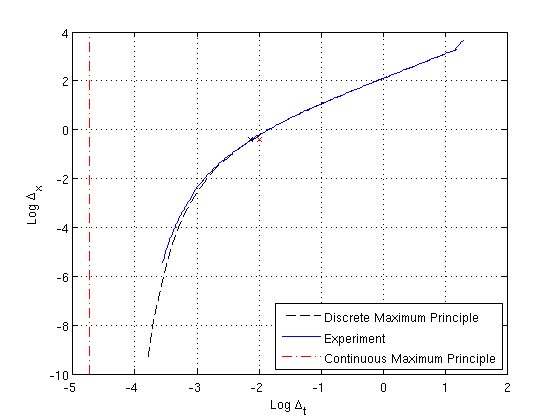
\includegraphics[width=0.7\linewidth]{CMP_DMP}
\caption{Continuous and Discrete Maximum Principles (see \cite{WolLarDen})}
\label{CMP_DMP}
\end{figure}


